%TODO no numeri a lato del codice
\begin{frame}[t,plain]
\titlepage
\end{frame}

\begin{frame}{Steps}
	\begin{itemize}
		\item Calibration
		\item Unwarping
		\item Detection
	\end{itemize}
\end{frame}


\begin{frame}{Calibration}
	Given a set of pictures taken with a camera, the object of this step is to find the camera matrix $A$ and the distortion coefficients $\dot{d}$.\newline
	\vfill
	\[
		A=\begin{bmatrix}
			f_x&0&c_x\\
			0&f_y&c_y\\
			0&0&1\\
		\end{bmatrix}\qquad
		\begin{matrix}
			x_{distorted}=x\left(1+k_1r^2+k_2r^4+k_3r^6\right)\\
			y_{distorted}=y\left(1+k_1r^2+k_2r^4+k_3r^6\right)\\
			x_{distorted}=x+\left[2p_1xy+p_2\left(r^2+2x^2\right)\right]\\
			y_{distorted}=y+\left[p_1\left(r^2+2y^2\right)+2p_2xy\right]\\
			\dot{d}=(k_1, k_2, p_1, p_2, k_3)
		\end{matrix}
	\]
	\vfill
\end{frame}


\begin{frame}{Calibration}
	\begin{figure}[H]
		\begin{minipage}{0.48\linewidth}
			\includegraphics[width=\linewidth]{Immagini/Chessboard1}
		\end{minipage}
		\vspace{0.04\linewidth}
		\begin{minipage}{0.48\linewidth}
			\includegraphics[width=\linewidth]{Immagini/Chessboard2}
		\end{minipage}
	\end{figure}
\end{frame}


\begin{frame}{Calibration}
	\begin{figure}[H]
		\begin{minipage}{0.48\linewidth}
			\includegraphics[width=\linewidth]{Immagini/Chessboard1Calibrated}
		\end{minipage}
		\vspace{0.04\linewidth}
		\begin{minipage}{0.48\linewidth}
			\includegraphics[width=\linewidth]{Immagini/Chessboard2Calibrated}
		\end{minipage}
	\end{figure}
	\stsize
	\[A=\begin{bmatrix}
		8.4247565095622963\times10^2 & 0 & 6.3709750745251142\times10^2\\
		0 & 8.4247565095622963\times10^2 & 4.9404840840221556\times10^2\\
		0 & 0 & 1
	\end{bmatrix}\]\[
	\dot{d}=(-2.5214446354851400\times10^{-1}, 7.2467634259951161\times10^{-2},\]\[-3.7212601356153754\times10^{-3}, 4.3313659139950872\times10^{-4}, 0)
	\]
\end{frame}

\begin{frame}{Unwarping}
Once the camera matrix and the distortion coefficients are known, the next step is to focus on the target, that is the circuit, and then to "un-distort" it. 
\begin{center}
	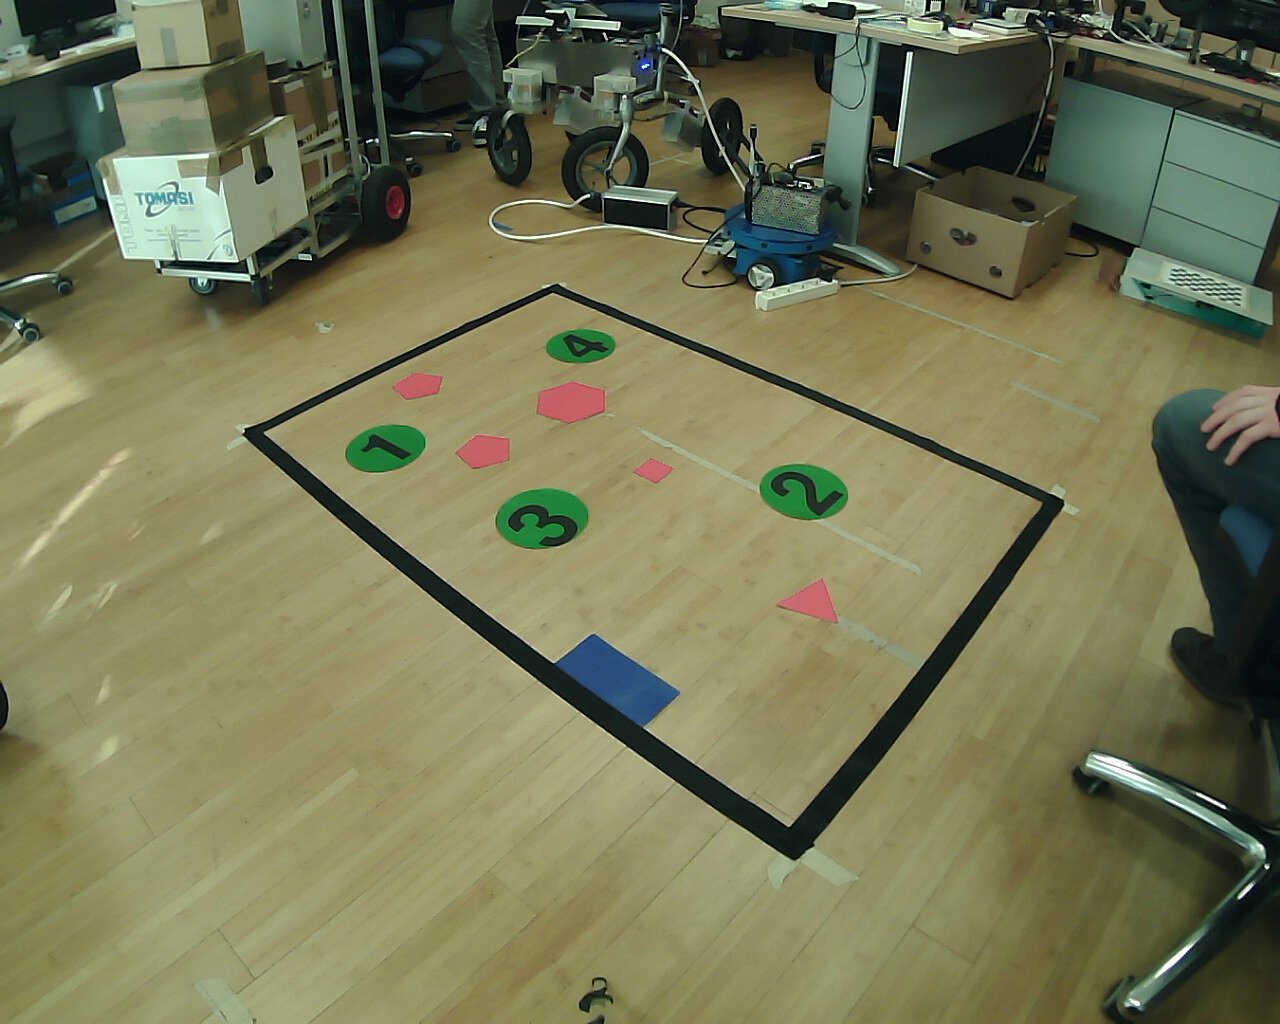
\includegraphics[scale=0.155]{Immagini/Wrapped.jpg}
\end{center}
\end{frame}

\begin{frame}{Unwarping}
	\begin{center}
		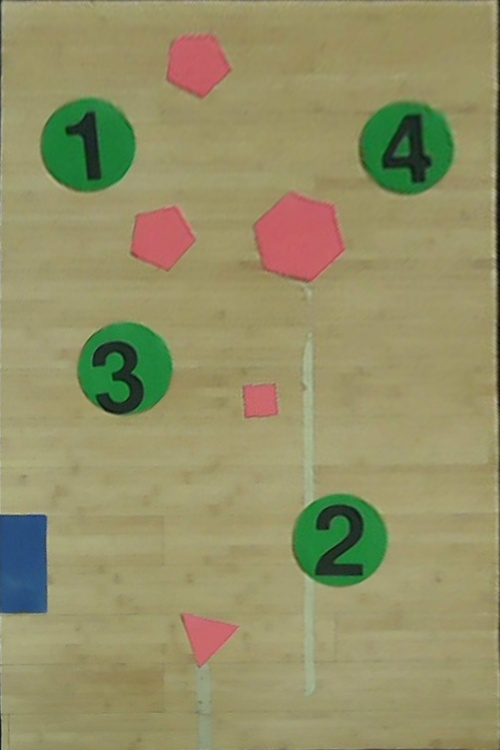
\includegraphics[scale=0.25]{Immagini/Unwrapped.jpg}
	\end{center}
\end{frame}

\begin{frame}[fragile]{Unwarping}
	Straighten the image using the distortion coefficients. 
	\begin{center}
		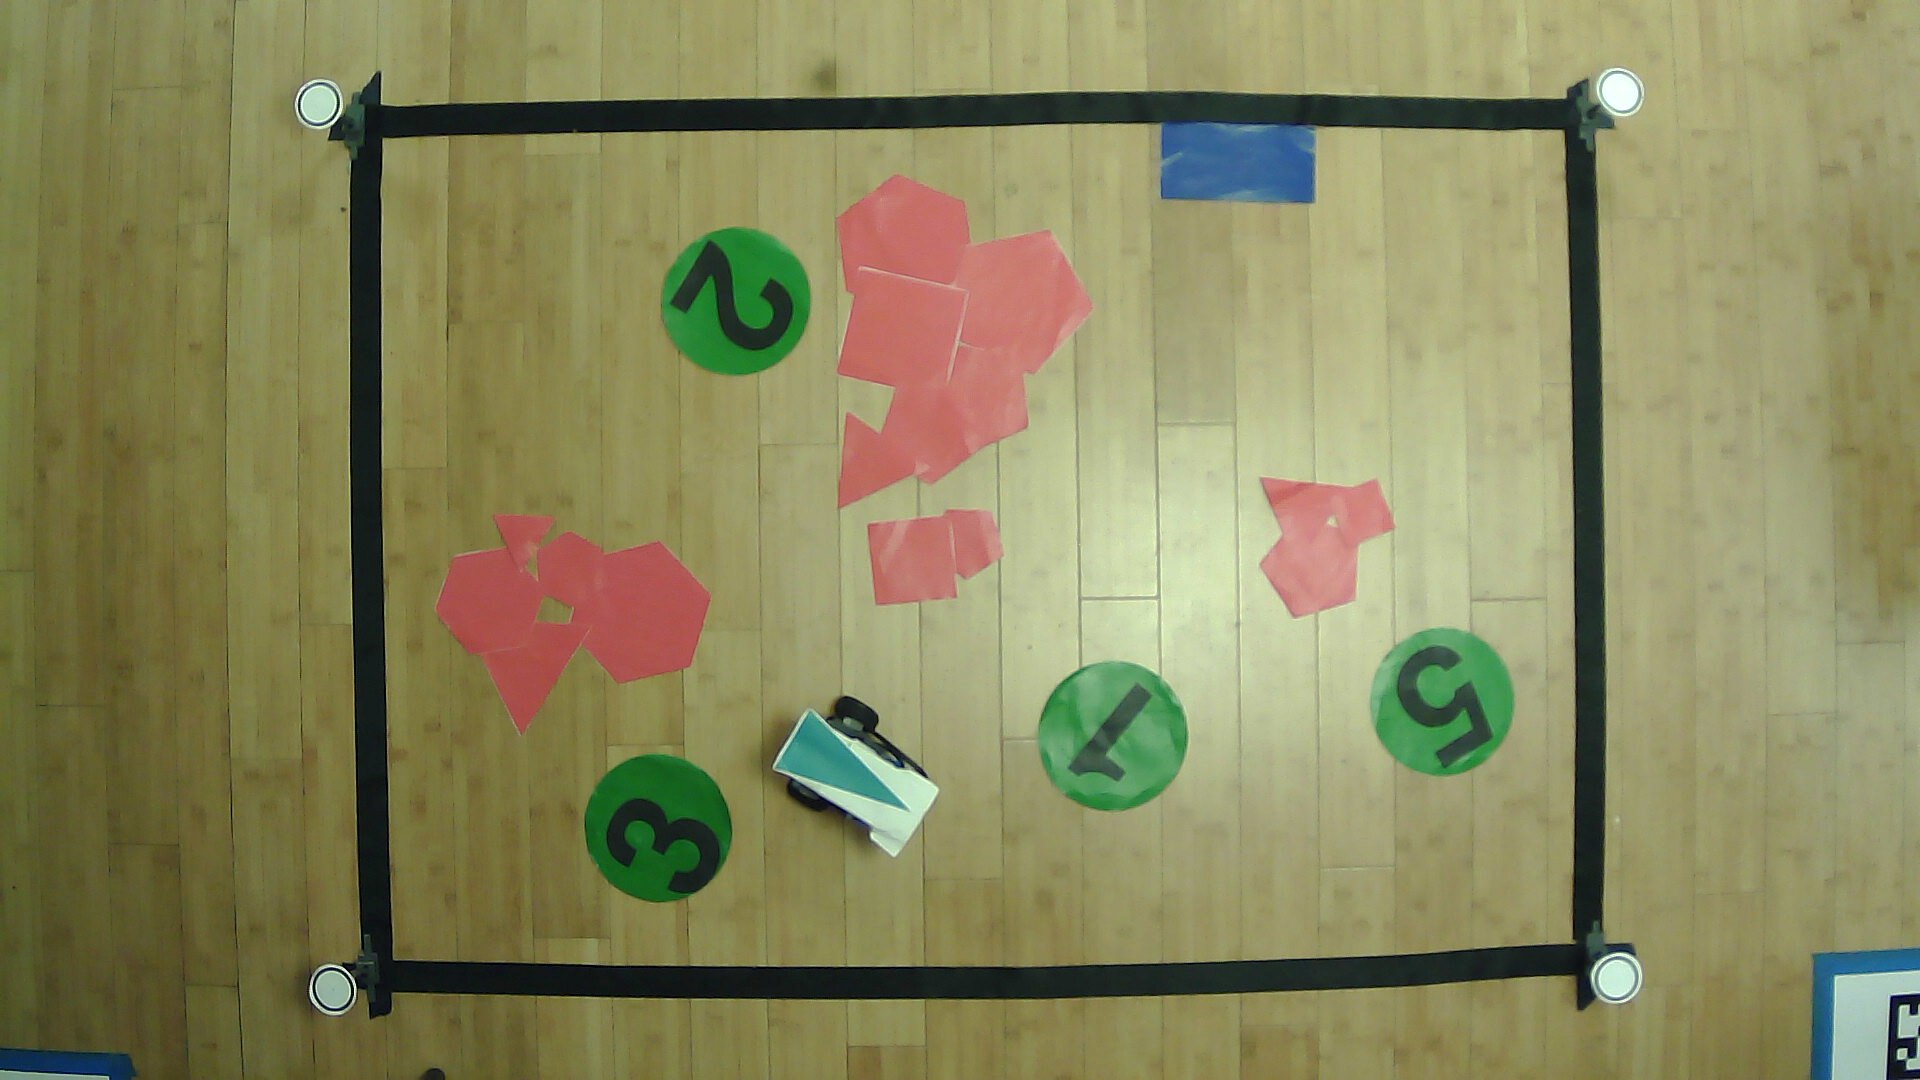
\includegraphics[scale=0.15]{Immagini/UNUndistort}	
	\end{center}
	\begin{minted}[fontsize=\stsize]{c++}
		loadCoefficients(calib_file, camera_matrix, dist_coeffs);
		undistort(or_img, fix_img, camera_matrix, dist_coeffs);
	\end{minted}
\end{frame}

\begin{frame}[fragile]{Unwarping}
	Then the image is converted from RGB to HSV.
	\begin{center}
		\includegraphics[scale=0.15]{Immagini/UNHSV}
	\end{center}
	\vfill
	\begin{minted}[fontsize=\stsize]{c++}
		cvtColor(fix_img, hsv_img, COLOR_BGR2HSV);
	\end{minted}
	\vfill
\end{frame}

\begin{frame}[fragile]{Unwarping}
	A black filter is added to highlight the black lines and areas.
	\begin{center}
		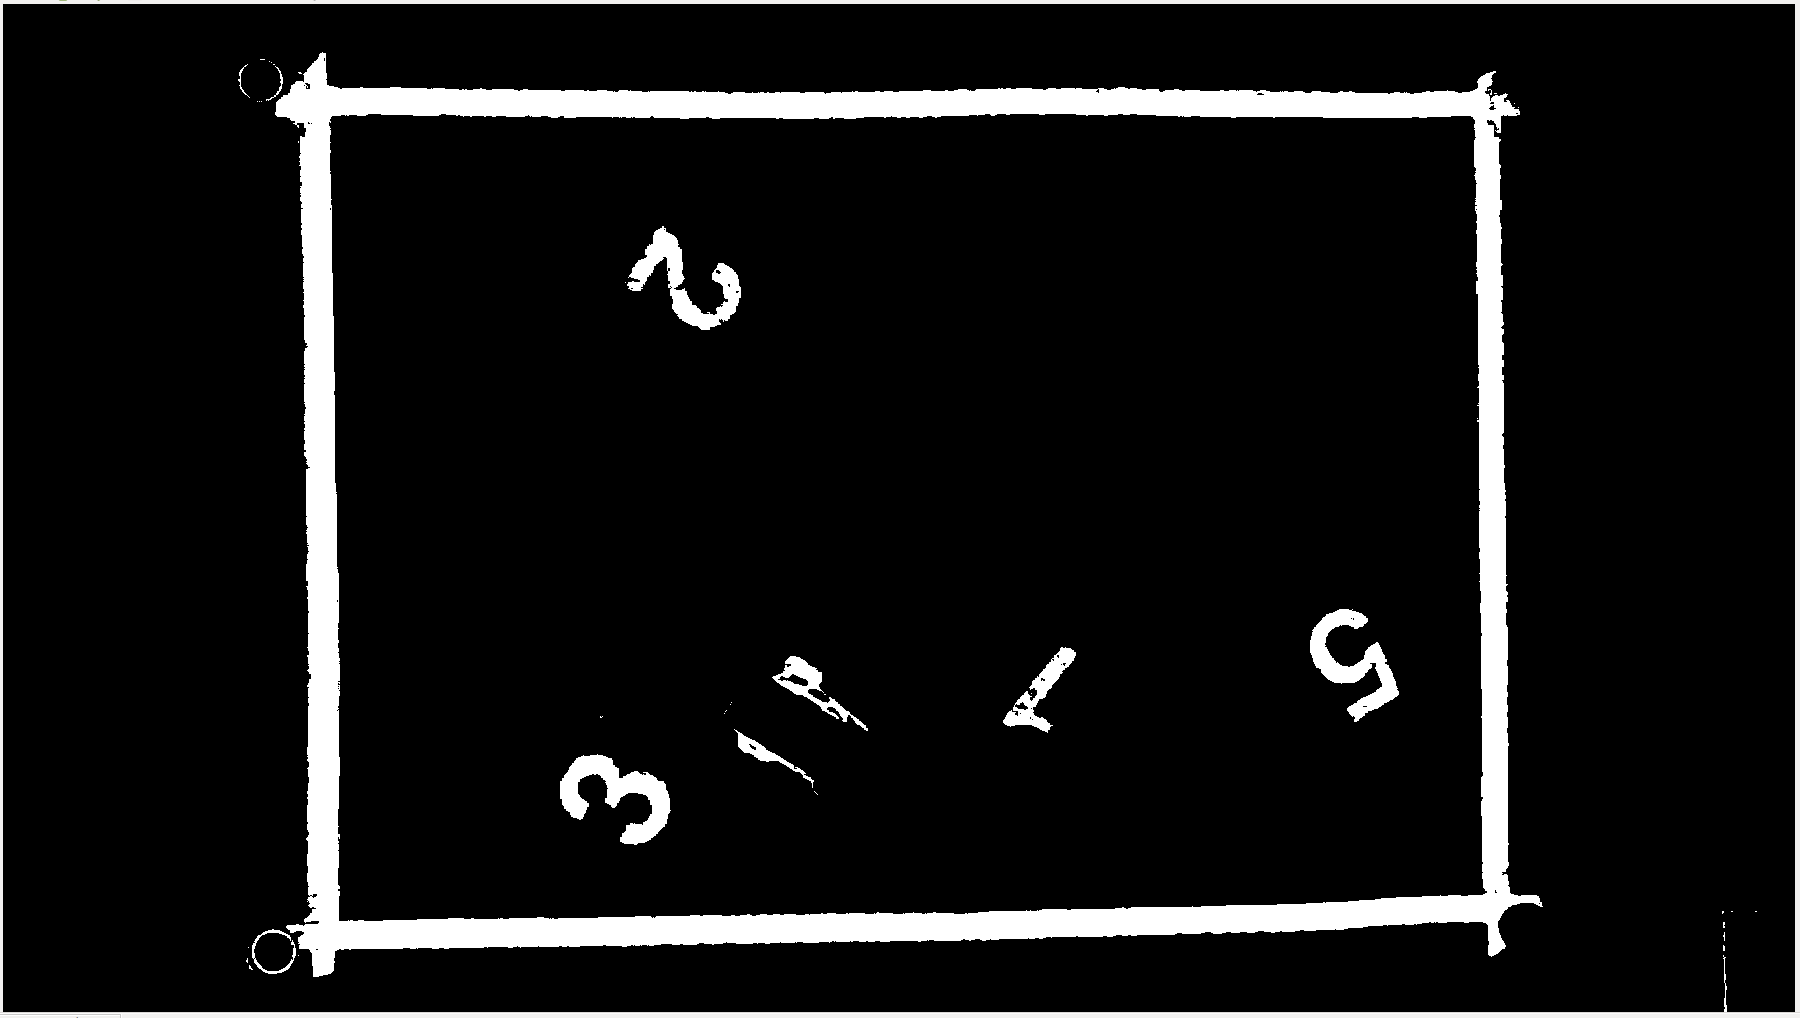
\includegraphics[scale=0.15]{Immagini/UNBlackFilter}
	\end{center}
	\vfill	
	\begin{minted}[fontsize=\stsize]{c++}
		FileNode Bm = fs_xml["blackMask"]; 
		//<blackMask>0 0 0 179 255 70</blackMask>
        inRange(hsv_img, Scalar(Bm[0], Bm[1], Bm[2]), Scalar(Bm[3], Bm[4], Bm[5]), black_mask);
	\end{minted}
	\vfill
\end{frame}

\begin{frame}[fragile]{Unwarping}
	Then the largest area enclosed by black lines is selected. 
	\begin{center}
		\includegraphics[scale=0.16]{Immagini/UNRect}
	\end{center}
\end{frame}

\begin{frame}[fragile]{Unwarping}
	At the end the image is cropped and turned. 
	\begin{center}
		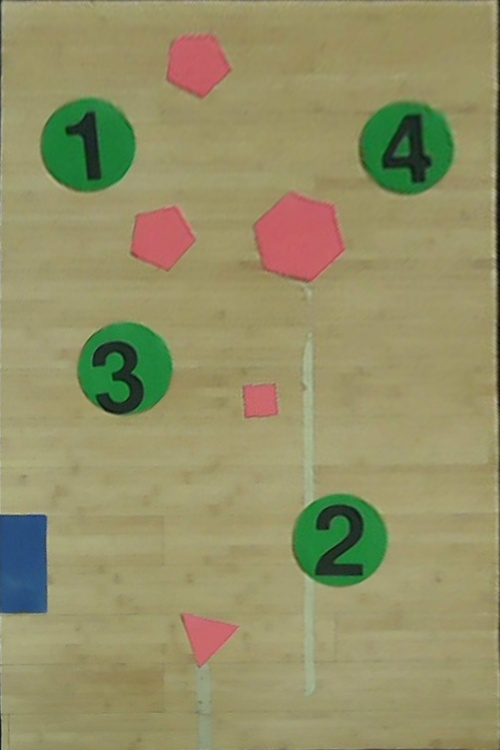
\includegraphics[scale=0.19]{Immagini/Unwrapped}
	\end{center}
\end{frame}


\begin{frame}[fragile]{Detection}
	The last phase consists of two more steps:
	\begin{itemize}
		\item Shape detection;
		\item Digit detection;
	\end{itemize}
\end{frame}

\begin{frame}[fragile]{Shape detection}
	The shape detection consists of scanning the image to locate the various obstacles, targets and the arriving point. \newline
	Various filer are here used to achieve this goal:
	\begin{itemize}
		\item The obstacles are red, so a red filter is going to be used: 15 100 140 160 255 255;
		\item The targets are green, so a green filter is going to be used: 50 65 45 70 255 200;
		\item The target point is blue, so a blue filter is going to be used: 100 100 40 140 200 170;
	\end{itemize}
	The various items are going to be stored in a file with the coordinates of their angles. 
\end{frame}

\begin{frame}{Shape detection}
	\begin{center}
		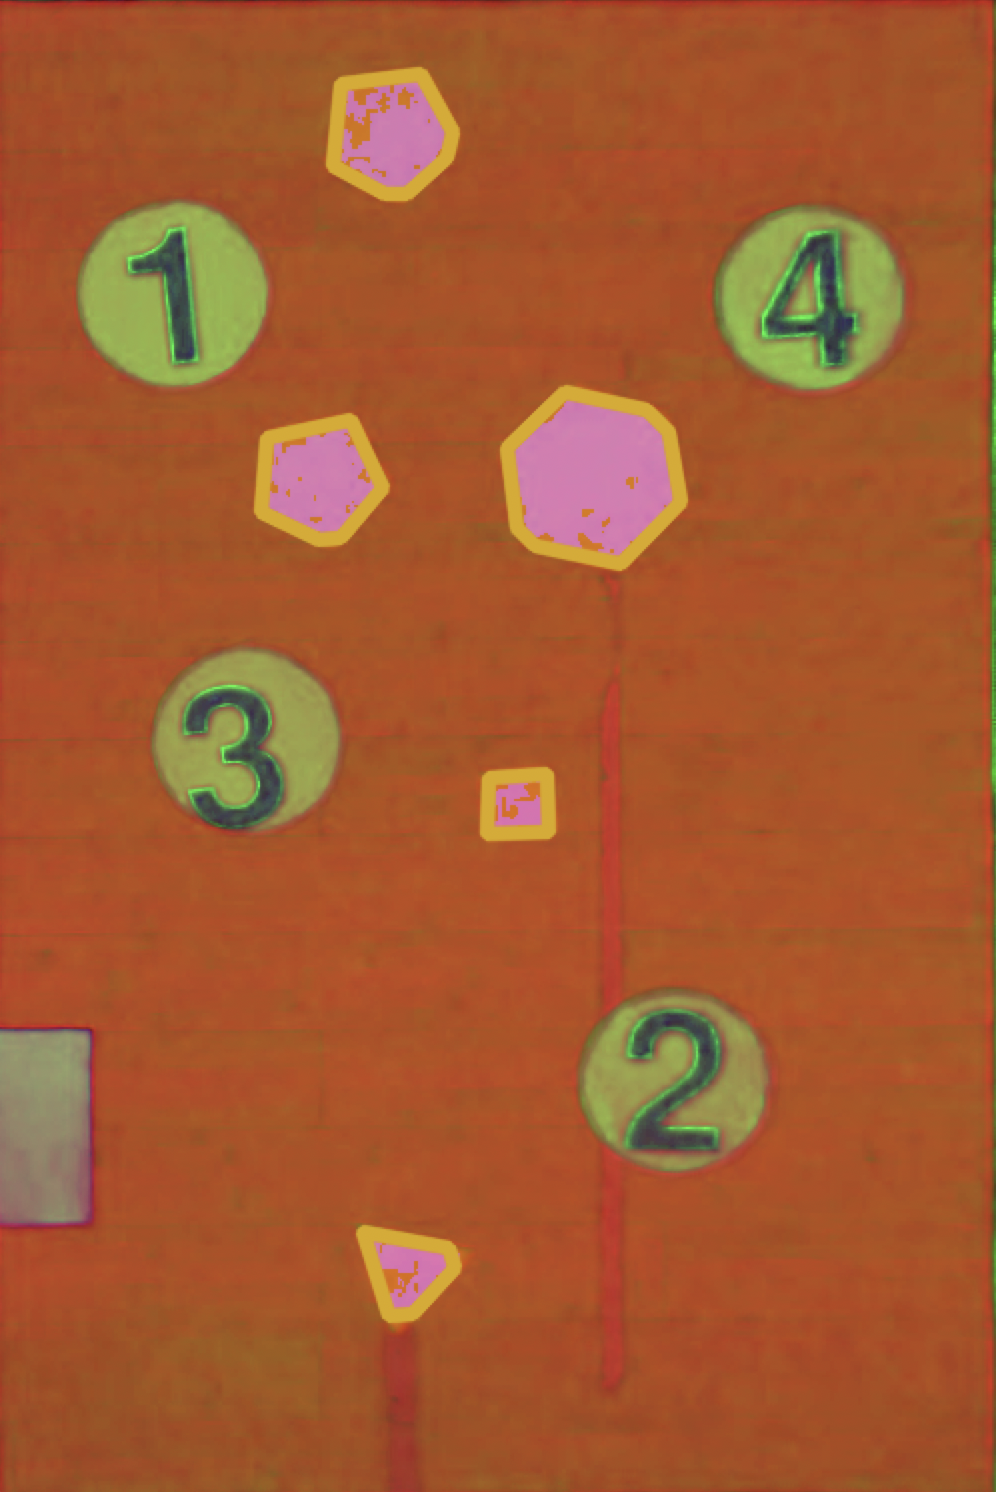
\includegraphics[scale=0.25]{Immagini/RedFiltered}
	\end{center}
\end{frame}

\begin{frame}[fragile]{Digit detection}
The goal of this last phase is to consider the area around the targets, which is our ROI, and try to identify the number inside it. \newline
This can be done through templates or through Tesseract API. 
For having better results the area around each target is:
\begin{itemize}
	\item Cropped;
	\item Resized to $200\times 200$ $px$;
	\item Given a black filter;
	\item Passed through a function (\mintinline{c++}{erode_dilation}) which aims to removing noise and isolate the number;
	\item Rotate so that the number is going to be vertical.
\end{itemize}
At last the digit detection is being done with templates since the success rate has been greater than using Tesseract. 
\end{frame}

%\begin{frame}{Code structure}
%	\begin{center}
%		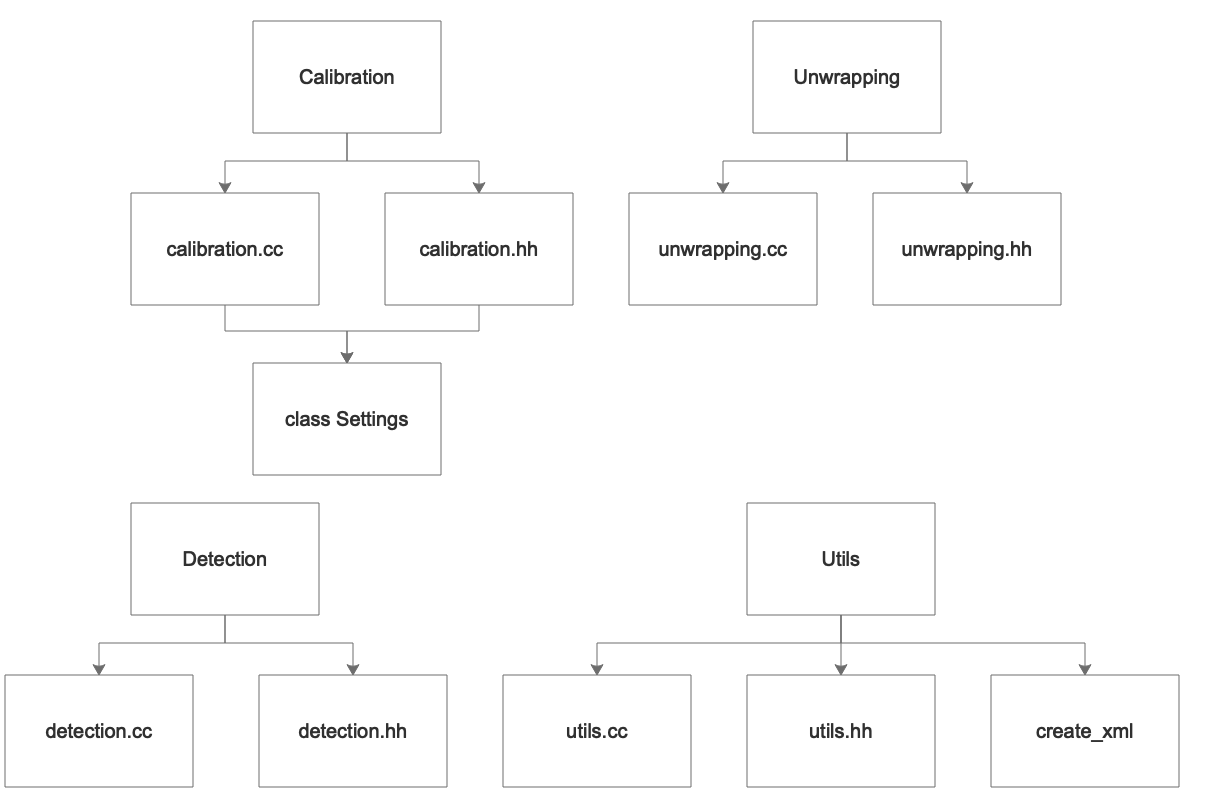
\includegraphics[scale=0.45]{Immagini/Code1}
%	\end{center}
%\end{frame}
%
%\begin{frame}{Code structure}
%	\begin{center}
%		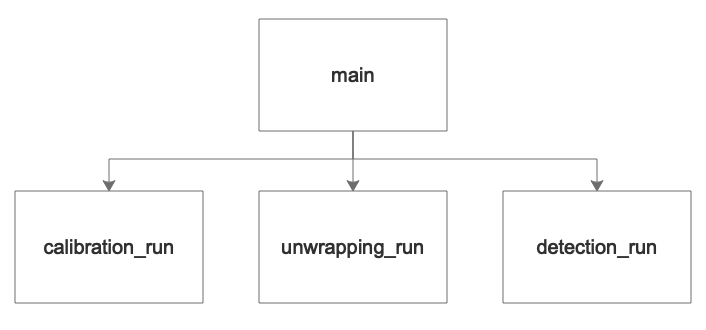
\includegraphics[scale=0.7]{Immagini/Code2}
%	\end{center}
%\end{frame}

